\documentclass[11pt,a4paper]{article}
\usepackage[margin=1in, headheight=14pt]{geometry}
\usepackage{amsfonts,amsmath,amssymb,suetterl}
\usepackage{lmodern}
\usepackage[T1]{fontenc}
\usepackage{fancyhdr}
\usepackage{float}
\usepackage[utf8]{inputenc}
\usepackage{fontawesome}
\usepackage{enumerate}
\usepackage{xcolor}
\usepackage{hyperref}
\usepackage{tikz}
\usepackage{nicefrac}
\usepackage{subcaption}
\usepackage{physics}
\usepackage{mathtools}
\usepackage{adjustbox}

\DeclareUnicodeCharacter{2212}{-}

\usepackage{mathrsfs}
\usepackage[nodisplayskipstretch]{setspace}

\setstretch{1.5}
\renewcommand{\footrulewidth}{0pt}

\parindent 0ex
\setlength{\parskip}{1em}
\raggedbottom

\begin{document}
      %
	\begin{center}
		\vspace*{8cm}
		\Huge MA202 –Differential Equations\\
		\LARGE LECTURE 19
  \end{center}
  \newpage
  %
	\section*{Periodic solutions and limit cycles}
	\begin{itemize}
		\item In this section we discuss further the possible existence of periodic solutions of second order autonomous systems
		$$
		\vb{x}^\prime = f(\vb{x})
		$$
		\item Such solutions satisfy the relation $\vb{x}(t + T) = \vb{x}(t)$ for all t and for some nonnegative constant T called the period.
		\item Periodic solutions are often important in physical problems because they represent phenomena that occur repeatedly.
		\item In many situations a periodic solution represents a “final state” toward which all “neighboring” solutions tend as the transients due to the initial conditions die out.
	\end{itemize}
	%
	\section*{Non-constant periodic solutions}
	\begin{itemize}
		\item Thus a periodic solution satisfies $\vb{x}(t + T) = \vb{x}(t)$ for all $t$ and for some nonnegative constant $T$.
		\item Note that a constant solution $x = x^0$ is periodic for any $T$.
		\item In this section, the periodic solutions that are discussed refer to nonconstant periodic solutions.
		\item In this case the period T is positive and is usually chosen as the smallest positive number for which $\vb{x}(t + T) = \vb{x}(t)$ is valid.
	\end{itemize}
	%
	\section*{Linear autonomous systems}
	\begin{itemize}
		\item Recall: The solutions of a linear autonomous system $\vb{x}^\prime = A\vb{x}$ are periodic if and only if the eigenvalues are pure imaginary.
		\item Thus if the eigenvalues of A are pure imaginary, then every solution of $\vb{x}^\prime = A\vb{x}$ is periodic, while if the eigenvalues of $A$ are not pure  imaginary, then there are no periodic solutions.
		\item The predator-prey equations to be discussed in Lecture 24, although nonlinear, behave similarly: All solutions in the first quadrant are periodic. See graph below.
		%
		\begin{figure}[H]
			\centering
			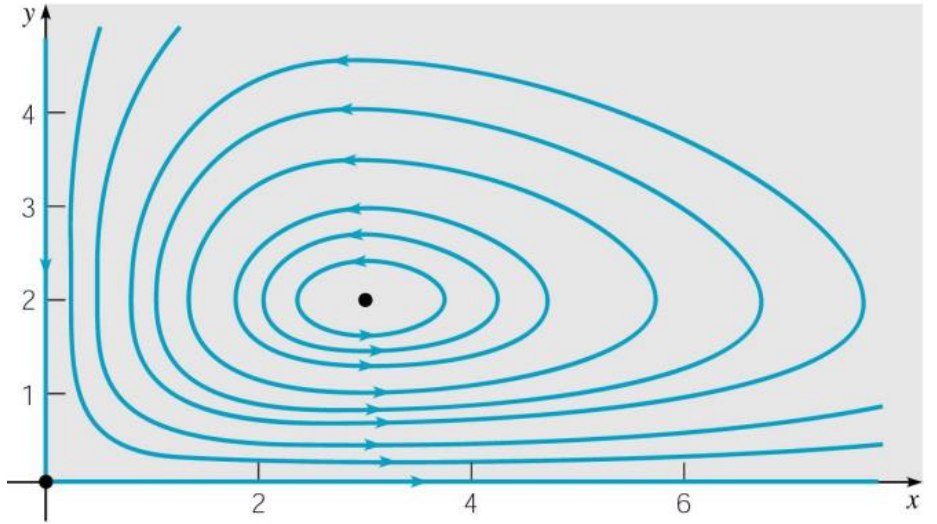
\includegraphics[width=0.55\textwidth]{figure/Lec19f1.PNG}
		\end{figure}
		%
	\end{itemize}
	%
	\section*{Example1: Nonlinear system (1 of 8)}
	\begin{itemize}
		\item Consider the nonlinear autonomous system
		$$
		\begin{pmatrix}
			x^\prime\\
			y^\prime
		\end{pmatrix}=
		\begin{pmatrix}
			x+y-x(x^2+y^2)\\
			-x+y-y(x^2+y^2)
		\end{pmatrix}
		$$
		\item It can be shown that $(0, 0)$ is the only critical point and that this system is almost linear near the origin.
		\item The corresponding linear system
		$$
		\begin{pmatrix}
			x^\prime\\
			y^\prime
		\end{pmatrix}=
		\begin{pmatrix}
			1 & 1\\
			-1 & 1
		\end{pmatrix}
		\begin{pmatrix}
			x\\
			y
		\end{pmatrix}
		$$
		has eigenvalues $1 \pm i$, and hence the origin is an unstable spiral point.
		%
		\begin{figure}[H]
			\centering
			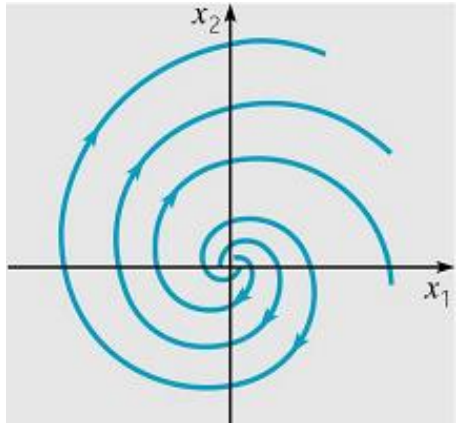
\includegraphics[width=0.55\textwidth]{figure/Lec19f2.PNG}
		\end{figure}
		%
	\end{itemize}
	%
	\section*{Example 1: Unstable spiral point (2 of 8)}
	\begin{itemize}
		\item Thus the origin is an unstable spiral point, and hence any solution that starts near the origin in the phase plane will spiral away from the origin.
		\item Since there are no other critical points, we might think that all solutions of our nonlinear system correspond to trajectories that spiral out to infinity.
		\item However, we will show that this is incorrect, because far away from the origin the trajectories are directed inward.
		%
		\begin{figure}[H]
			\centering
			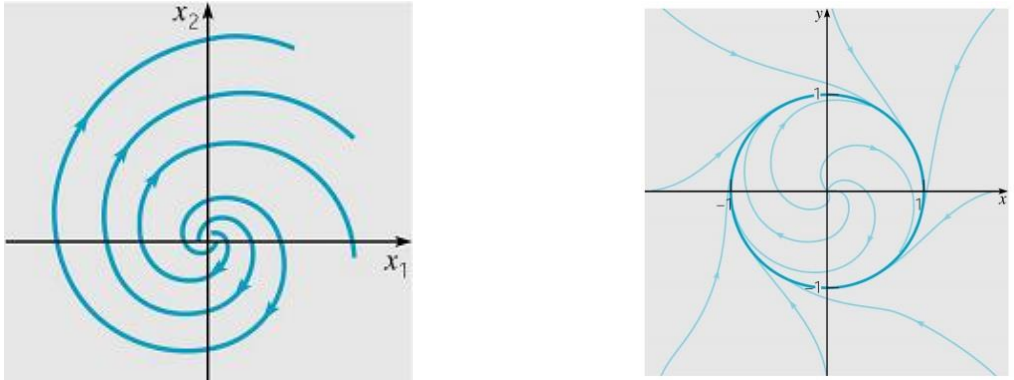
\includegraphics[width=0.85\textwidth]{figure/Lec19f3.PNG}
		\end{figure}
		%
	\end{itemize}
	%
	\section*{Example 1: Polar coordinates (3 of 8)}
	\begin{itemize}
		\item Our nonlinear system can be written as
		$$
		dx/dt = x+y-x(x^2+y^2),\ dy/dt = -x+y-y(x^2+y^2)
		$$
		\item Then
		$$
		x\frac{dx}{dt} + y\frac{dy}{dt} = x^2 + xy - x^2(x^2+y^2)^2
		$$
		\item Using polar coordinates $x = r \cos\theta\ \text{and}\ y = r\sin\theta $, note that
		$$
		r^2 = x^2+y^2,\ \text{and}\ r\frac{dr}{dt} = x\frac{dx}{dt} + y\frac{dy}{dt}
		$$
		\item Thus
		$$
		r\frac{dr}{dt} = r^2(1-r^2)
		$$
	\end{itemize}
	%
	\section*{Example 1: Critical points for equation of radius (4 of 8)}
	\begin{itemize}
		\item The critical points (for $r \geq 0$) of
		$$
		r(dr/dt) = r^2(1-r^2)
		$$
		are $r = 0$ (the origin) and $r = 1$, which corresponds to the unit circle in the phase plane.
		\item Note that $dr/dt > 0$ if $r < 1$ and $dr/dt < 0$ if $r > 1$. Thus inside the unit circle, the trajectories are directed outward, while outside the unit circle they are directed inward.
		\item The circle $r = 1$ looks like a limiting trajectory for the system.
		\item We next determine an equation for $\theta$.
		%
		\begin{figure}[H]
			\centering
			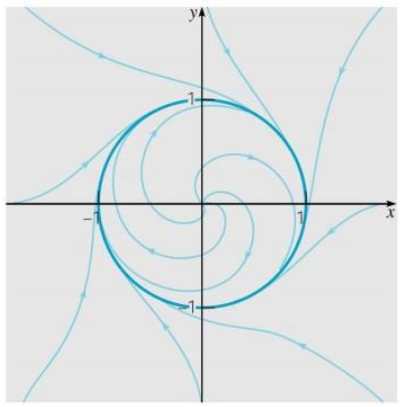
\includegraphics[width=0.55\textwidth]{figure/Lec19f4.PNG}
		\end{figure}
		%
	\end{itemize}
	%
	\section*{Example 1: Equation for angle (5 of 8)}
	\begin{itemize}
		\item Recall our nonlinear system:
		$$
		dx/dt = x+y-x(x^2+y^2),\ dy/dt = -x+y-y(x^2+y^2)
		$$
		\item Then
		$$
		y\frac{dx}{dt} - x\frac{dy}{dt} = xy + y^2 - xy(x^2+y^2) + x^2 - xy + xy(x^2+y^2) = (x^2+y^2)
		$$
		\item Using polar coordinates $x = r\cos\theta $ and $y = r\sin\theta$, note that
		$$
		r^2 = x^2+y^2,\ \frac{dx}{dt} = -r\sin\theta \frac{d\theta}{dt} = -y\frac{d\theta}{dt},\ \frac{dy}{dt} = r\cos \theta\frac{d\theta}{dt} = x\frac{d\theta}{dt}
		$$
		\item It follows that
		$$
		-y^2\frac{d\theta}{dt}-x^2\frac{d\theta}{dt} = r^2 \Leftrightarrow -r^2\frac{d\theta}{dt} = r^2 \Leftrightarrow \frac{d\theta}{dt} = -1
		$$
	\end{itemize}
	%
	\section*{Example 1: A solution to polar equations (6 of 8)}
	\begin{itemize}
		\item Our original nonlinear system
		$$
		dx/dt = x+y-x(x^2+y^2),\ dy/dt = -x+y-y(x^2+y^2)
		$$
		is therefore equivalent to the system
		$$
		r(dr/dt) = r^2(1-r^2),\ d\theta/dt = -1
		$$
		\item One solution to this system is
		$$
		r = 1,\ \theta = -t+t_0
		$$
		where $t_0$is an arbitrary constant.
		\item As $t$ increases, a point on this solution trajectory moves clockwise around the  unit circle.
		%
		\begin{figure}[H]
			\centering
			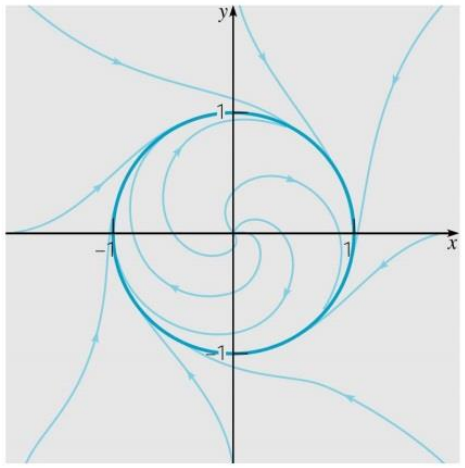
\includegraphics[width=0.55\textwidth]{figure/Lec19f5.PNG}
		\end{figure}
		%
	\end{itemize}
	%
	\section*{Example 1: General solution to polar equations (7 of 8)}
	\begin{itemize}
		\item Other solutions of 
		$$
		r\frac{dr}{dt} = r^2(1-r^2)
		$$
		can be found by separation of variables: For $r \neq 0$ and $r \neq 1$,
		$$
		\frac{dr}{r(1-r^2)} = dt,
		$$
		and after using a partial fraction expansion and some algebra,
		$$
		r = \frac{1}{\sqrt{1+c_0e^{-2t}}},\ \theta = -t + t_0
		$$
		where $c_0$ and $t_0$ are arbitrary constants.
		\item Note that $c_0 = 0$ yields $r = 1, \theta = -t + t_0$, as before.
	\end{itemize}
	%
	\section*{Example 1: Initial value problem in polar form (8 of 8)}
	\begin{itemize}
		\item The solution satisfying the initial value problem
		$$
		r\frac{dr}{dt} = r^2(1-r^2),\ \frac{d\theta}{dt} = -1;\ r(0) = \rho,\ \theta(0) = \aleph
		$$
		is given by
		$$
		r = \frac{1}{\sqrt{1 + [(1/\rho^2)-1]e^{-2t}}},\ \theta = -(t-\alpha)
		$$
		\item We have the following two cases:
		\begin{itemize}
			\item[\labelitemi] If $\rho < 1$, then $r \to 1$ from the inside as $t \to \infty$.
			\item[\labelitemi] If $\rho > 1$, then $r \to 1$ from the inside as $t \to \infty$.
		\end{itemize}
		\item See the phase portrait on the right.
	\end{itemize}
	%
	\section*{Limit cycle}
	\begin{itemize}
		\item In the previous example, the circle $r = 1$ not only corresponds to periodic solutions of the system
		$$
		dx/dt = x+y-x(x^2+y^2),\ dy/dt = -x+y-y(x^2+y^2)
		$$
		but it also attracts other nonclosed trajectories that spiral toward it as $t \to \infty$
		\item In general, a closed trajectory in the phase plane such that other nonclosed trajectories spiral toward it, either from the inside or the outside, as $t \to \infty$, is called a \textbf{limit cycle}.
		%
		\begin{figure}[H]
			\centering
			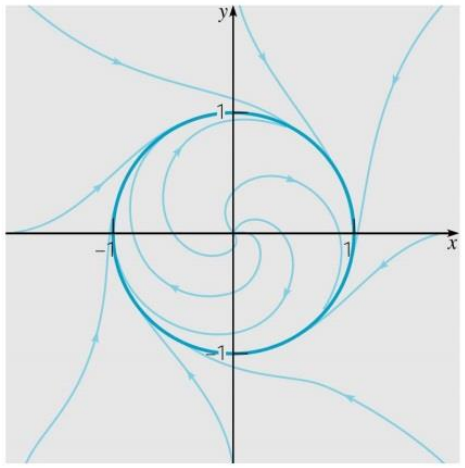
\includegraphics[width=0.55\textwidth]{figure/Lec19f5.PNG}
		\end{figure}
		%
	\end{itemize}
	\section*{Stability of closed trajectories}
	\begin{itemize}
		\item If all trajectories that start near a closed trajectory spiral toward the closed trajectory as $t \to \infty$, both from the inside and the outside, then the limit cycle is \textbf{asymptotically stable}.
		\item In this case, since the closed trajectory is itself a periodic orbit rather than an equilibrium point, this type of stability is often called \textbf{orbital stability}.
		\item If the trajectories on one side spiral toward a closed trajectory , while those on the other side spiral away as $t \to \infty$, then the closed trajectory is \textbf{semistable}.
		\item If the trajectories on both sides of a closed trajectory spiral away as $t \to \infty$, then the closed trajectory is \textbf{unstable}.
		\item Closed trajectories for which other trajectories neither approach nor depart from are called \textbf{stable}.		
	\end{itemize}
	%
	\section*{Theorem 9.7.1}
	\begin{itemize}
		\item Consider the autonomous system
		$$
		dx/dt = F(x,y),\ dy/dt = G(x,y),
		$$
		\item Let $F$ and $G$ have continuous first partial derivatives in a domain $D$ in the $xy$-plane.
		\item A closed trajectory of the system must necessarily enclose at least one critical (equilibrium) point.
		\item If it encloses only one critical point, the critical point cannot be a saddle point.
		\item \textcolor{red}{Note:} It follows that in any region not containing a critical point, there cannot be a closed trajectory within that region. 		
	\end{itemize}
	%
	\section*{Theorem 9.7.2}
	\begin{itemize}
		\item Consider the autonomous system
		$$
		dx/dt = F(x,y),\ dy/dt = G(x,y),
		$$
		\item Let $F$ and $G$ have continuous first partial derivatives in a simply connected domain $D$ in the $xy$-plane.
		\item If $F_x + G_y$ has the same sign throughout $D$, then there is no closed trajectory of the system lying entirely within $D$.
		\item \textcolor{red}{Note:} A simply connected domain in the $xy$-plane is a domain with no holes.
		\item Also, If $F_x + G_y$ changes sign in $D$, then no conclusion can be drawn.
	\end{itemize}
	%
	\section*{Example 2: Applying Theorem 9.7.2 (1 of 2)}
	\begin{itemize}
		\item Consider again the nonlinear autonomous system of Example
		$$
		dx/dt = x+y-x(x^2 + y^2),\ dy/dt = -x+y-y(x^2+y^2)
		$$
		\item Then $F_x + G_y = 2-4(x^2+y^2) = 2(1-2r^2)$
		\item Thus $F_x + G_y > 0$ on $0 \leq r < (1/2)^{\nicefrac{1}{2}}$, so there is no closed trajectory in this simply connected circular disk.
		\item From the first example, there is no closed trajectory in $r < 1$.
		\item Thus the information given in Theorem 9.7.2 may not be the best possible result.
		%
		\begin{figure}[H]
			\centering
			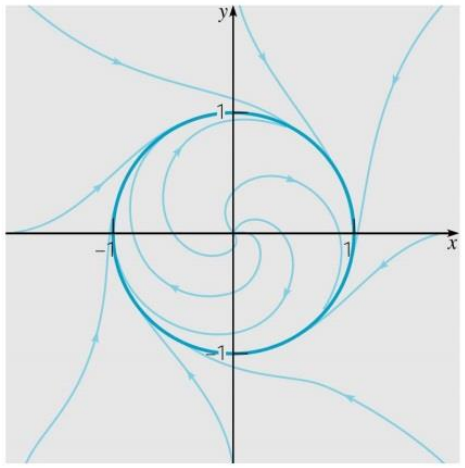
\includegraphics[width=0.55\textwidth]{figure/Lec19f5.PNG}
		\end{figure}
		%
	\end{itemize}
	%
	\section*{Example 2: Annular region and Theorem 9.7.2 (2 of 2)}
	\begin{itemize}
		\item Note that
		$$
		F_x + G_y = 2(1-2r^2)<0\ \text{on}\ r>1/\sqrt{2}
		$$
		\item However, Theorem 9.7.2 does not apply since the annular region $r > (1/2)^{\nicefrac{1}{2}}$ is not simply connected.
		\item Thus we cannot use Theorem 9.7.2 to conclude that there is no closed trajectory lying entirely within $r > (1/2)^{\nicefrac{1}{2}}$.
		\item In fact, from the first example, we know that $r = 1$ is a closed trajectory for the system that lies entirely within $r > (1/2)^{\nicefrac{1}{2}}$.
		%
		\begin{figure}[H]
			\centering
			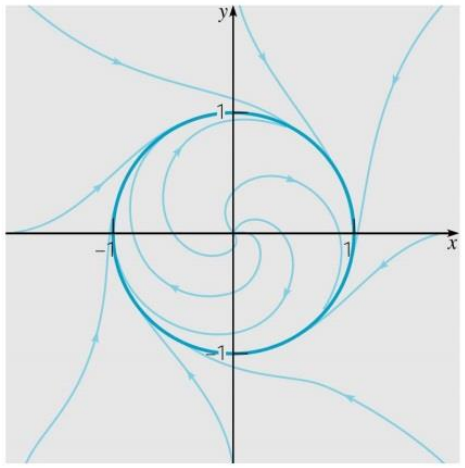
\includegraphics[width=0.55\textwidth]{figure/Lec19f5.PNG}
		\end{figure}
		%
	\end{itemize}
	%
	\section*{Theorem 9.7.3 (Poincar\'{e}-Bendixson)}
	\begin{itemize}
		\item Consider the autonomous system
		$$
		dx/dt = F(x,y),\ dy/dt = G(x,y),
		$$
		\item Let $F$ and $G$ have continuous first partial derivatives in a domain $D$ in the $xy$-plane.
		\item Let $D_1$ be a bounded subdomain in $D$, and let $R$ be the region that consists of $D_1$ plus its boundary (all points of $R$ are in $D$).
		\item Suppose that $R$ contains no critical point of the system.
		\item If there exists a constant $t_0$ such that $x = \phi(t),\ y = \psi(t)$ is a solution of the system that exists and stays in $R$ for all $t > t_0$, then $x = \phi(t),\ y=\psi(t)$ either is a periodic solution (closed trajectory) or spirals toward a closed trajectory as $t \to \infty$.
		\item In either case, the system has a periodic solution in $R$.
	\end{itemize}
	%
	\section*{Example 3: Applying Theorem 9.7.3}
	\begin{itemize}
		\item Example 3: Applying Theorem 9.7.3
		$$
		dx/dt = x+y-x(x^2+y^2),\ dy/dt = -x+y-y(x^2+y^2)
		$$
		\item Since the origin is a critical point, it must be excluded from $R$.
		\item Consider the region $R$ defined by $0.5 \leq r \leq 2$.
		\item Recall from the first example $dr/dt = r(1-r)$ for $0.5 \leq r \leq 2$.
		\item For $r = 0.5$, $dr/dt > 0$ and hence $r$ increases, while for $r = 2$, $dr/dt < 0$ and hence $r$ decreased.
		\item Thus a trajectory that crosses the boundary of $R$ is entering $R$.
		\item Consequently, any solution that starts in $R$ at $t = t_0$ cannot leave but must stay in $R$ for all $t > t_0$, and is either a periodic solution or approaches one as $t \to \infty$.
		%
		\begin{figure}[H]
			\centering
			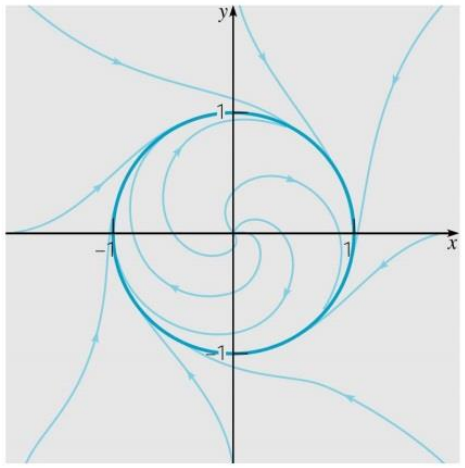
\includegraphics[width=0.55\textwidth]{figure/Lec19f5.PNG}
		\end{figure}
		%
	\end{itemize}
\end{document}